\chapter{Security Issues}

EAP is a standard that provides an infrastructure for network access clients and authentication servers. EAP does not specify the authentication mechanism itself but the way it is negotiated by the communicating parties. Consequently, EAP has no security issues in itself. In contrast, each EAP implementation stipulates some specific valid authentication methods. Consequently, EAP implementations may furnish with security vulnerabilities. The following section summarize security issues associated EAP.

\section{EAP Protocol Vulnerabilities}
\subsection{TLS Based EAP protocols}
\subsection{Transport Layer Security [TLS]}
Transport Layer Security (TLS) and its predecessor, Secure Socket Layer (SSL) are cryptographic protocols that provide secure communication on the Internet for secure web browsing, e-mail, Internet faxing, instant messaging and other data transfers. The protocol allows client/server applications to communicate in a way that is designed to prevent eavesdropping, tampering, or message forgery. For example, HTTPS protocol layers on top of TLS protocol to protect sensitive network traffic.TLS is a layered protocol, and consists of the Record protocol, the Alert protocol and the Handshake protocol. The Record protocol is designed to serve the Handshake protocol and Alert protocol, and offers symmetric encryption, data authenticity, and optionally compression. The Alert protocol offers some signaling to the other protocols and between peers. An alert signal includes an alert level indication, and a FATAL ALERT always terminates the current connection. The Handshake protocol is responsible for the cipher suite
negotiation, the initial key exchange, and the authentication of the two peers. In our attack we mainly attack the Handshake protocol by triggering the alert messages defined in the Alert protocol. Figure 3 shows the flowchart of a successful TLS handshake process. Generally, the TLS server starts the procedure and the client responds with a hello message. The server then sends its certificate, selected cipher suit and so on. Note that TLS provides an option to authenticate the client as well by requesting the client certificate. The client returns selected
cipher, its certificate (optional) and other cryptographic information. Note in Figure 3, we put some messages close
as if bundled together because they may be embedded in a single EAP packet, depending on the message sizes. 

\begin{figure}[htb]
\centering	
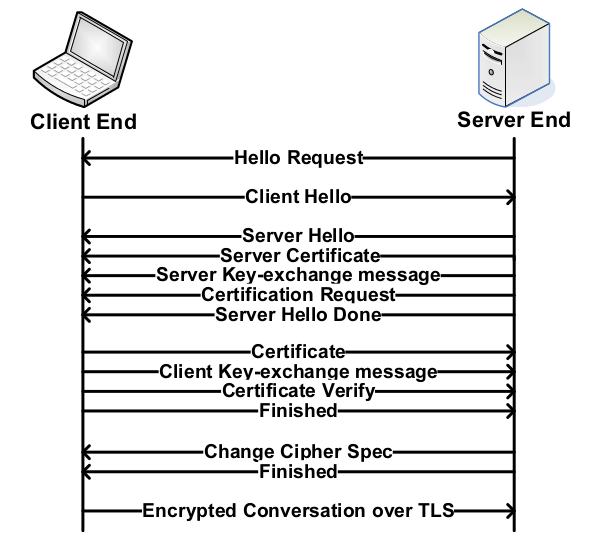
\includegraphics[width=.9\textwidth]{images/EAP_TLS.png}
\caption{EAP TLS Handshake} 
\label{fig:EAP TLS Handshake}
\end{figure}

\subsection{Vulnerability in TLS based EAP Protocols}


\subsection{EAP-SIM Weakness}
EAP-SIM is designed to provide security enhancements to the GSM authentication, it does not meet its
security goals. If an attacker wants to authenticate himself to a mobile user and impersonate an AAA server, the only thing that he has to do is to generate a valid keyed MAC using a K-auth key. A valid MAC can be generated by possessing two or three Kc keys and the related RAND parameters of GSM authentication triplets, which can be obtained with one of the following ways:\newline
1. Having physical access to a SIM card, it is easy to obtain any parameter of GSM triplets.\newline
2. Using virus or other malicious piece of software, an adversary may mount an attack on the user platform in
order to obtain triplets. \newline
3. If the same SIM credentials are also used for GSM traffic, the triplets could be revealed in the GSM network.\newline
4. An attacker could gain access to the communication between the AuC and the AAA server in the EAP-SIM
authentication dialogue. \newline
Thus, if eventually multiple GSM triplets are compromised;then, an adversary may impersonate a valid network and start an authentication session with the mobile user. The attacker can calculate a valid hashed MAC, as he possesses the RAND parameters, and he can generate the K-auth from the encryption keys Kc. Since there is no way for the user to understand that there is an attack, he authenticates the attacker as a legitimate network, based on the received valid MAC.
The compromised GSM triplets can be used by an adversary to perform attacks as long as the permanent key Ki, which is employed to produce the triplets, remains the same and this could be for years. This is one example of attacks. 
There are two other type of attacks on EAP-SIM which we will discuss in more detail. 
